\chapter{Background and Related Works}
\label{ch:background}
\section{Literature Review}
For decades, researchers attempt to reveal the rules behind stock price's changing. Their works can be categorized into two basic groups: (1) directly predicting stock price, including using traditional ``technical analysis'', neural network and fuzzy time-series, etc.; (2) extracting interesting patterns/turning points for decision making, including using clustering algorithms and charts, etc. In this project, we focus on works that mainly utilizes clustering algorithms to find the similarity in stock trends. Similar to other time-series data, stock price data are long sequences with varying length, therefore, they cannot be directly analyzed.
To make the analysis tractable, \cite{fu2001pattern} proposed a pattern discovery framework for stock time series, which includes three phases: (1) segmentation phase: split intractable long sequences into smaller fragments; (2) clustering phase: group the fragments into clusters, the centroids of clusters are regarded as unique patterns; (3) matching phase: use pattern matching algorithms to find matches of the generated patterns in test data. To mitigate the time complex problem brought by the length of patterns, they used a perceptually important point (PIP) identification algorithm to compress the data. 
\cite{basalto2005clustering} used chaotic map clustering (CMC) algorithm to identify the temporal patterns of the stock prices, each company/stock is assigned to a map, and similarity between stocks/companies were measured by the coupling strengths between maps, their work proved that co-movement of stock price exists in the same industrial branch. \cite{liao2008mining} studied on the association between stocks and used K-means algorithm to group stocks, they proved that similar stock price fluctuation can happen within geographic regions. \cite{chen2016intelligent} manually defined a stock price pattern called PIP bull-flag based on the pattern defined by \cite{leigh2002stock,leigh2002forecasting}, proposed two matching algorithms to find pre-defined patterns (a timing on the stock series), and used template matching technique to help investment strategy making. \cite{nanda2010clustering} examined the performance of K-means, SOM and Fuzzy C-means clustering algorithms on stock data with 9 evaluation criteria, and found that the clusters generated by K-means were the most compact. \cite{aghabozorgi2014stock} argued that previous one-phase approaches can not deep into smaller granularity, and proposed a three-phase clustering method for stock clustering: (1) approximate clustering; (2) purifying and summarization; (3) merging. \cite{kong2020pattern} used the trajectories before stock price jumps rather than the whole data series to classify stocks, and found that the patterns around turning points are more guiding.

\section{Related Works}
This section gives a brief review of techniques used in this project, including time-series data compression, path signature, and clustering algorithms.

\subsection{Time-series data compression}
Stock price records are typical time-series data, and they have natures such as large data volume, high dimensionality, etc. Analyzing the raw data may need huge computing resource, therefore, in most algorithms, the data are compressed. There are several methods to reduce the dimension of the original data, simple approaches include: (1) simpling \cite{aastrom1969choice}, which randomly selects n points from a time series (n is the dimension after compression); (2) piecewise aggregate approximation (PAA) \cite{keogh2001dimensionality,yi2000fast}, which segments the time series into n sub trajectories, and uses the numerical mean of each trajectory to represent the whole time series.
\\More promising methods aim to use the perceptually important points (PIP) to represent the time series \cite{fu2011review}. The PIP identification algorithm is first proposed by \cite{chung2001flexible} and then used wildly in time series data analysis. Given a time series $ P = \{P_1, P_2, \cdots, P_k\}$, where $P_t \in P$ is a data point, PIP identification process will calculate the importance of all the data points, and the first n points with higher importance will be used to represent the whole series. This process works as follows: the start point $P_1$ and the end point $P_2$ in $P$ are the first two PIPs. The third point will be the one with maximum distance to the first two PIPs. The order of remaining PIPs will be decided by their vertical distance to the line crossing its two adjacent PIPs. This process continues until n PIPs are found (n is the reduced dimension) or all points in $P$ are ordered. Figure \ref{fig:ppa} and \ref{fig:pip} show the compression results of PPA and PIP algorithms respectively.
\begin{figure}[!htbp]
    \label{fig:compression}
    \centering
    \subfigure[Original time series]{
        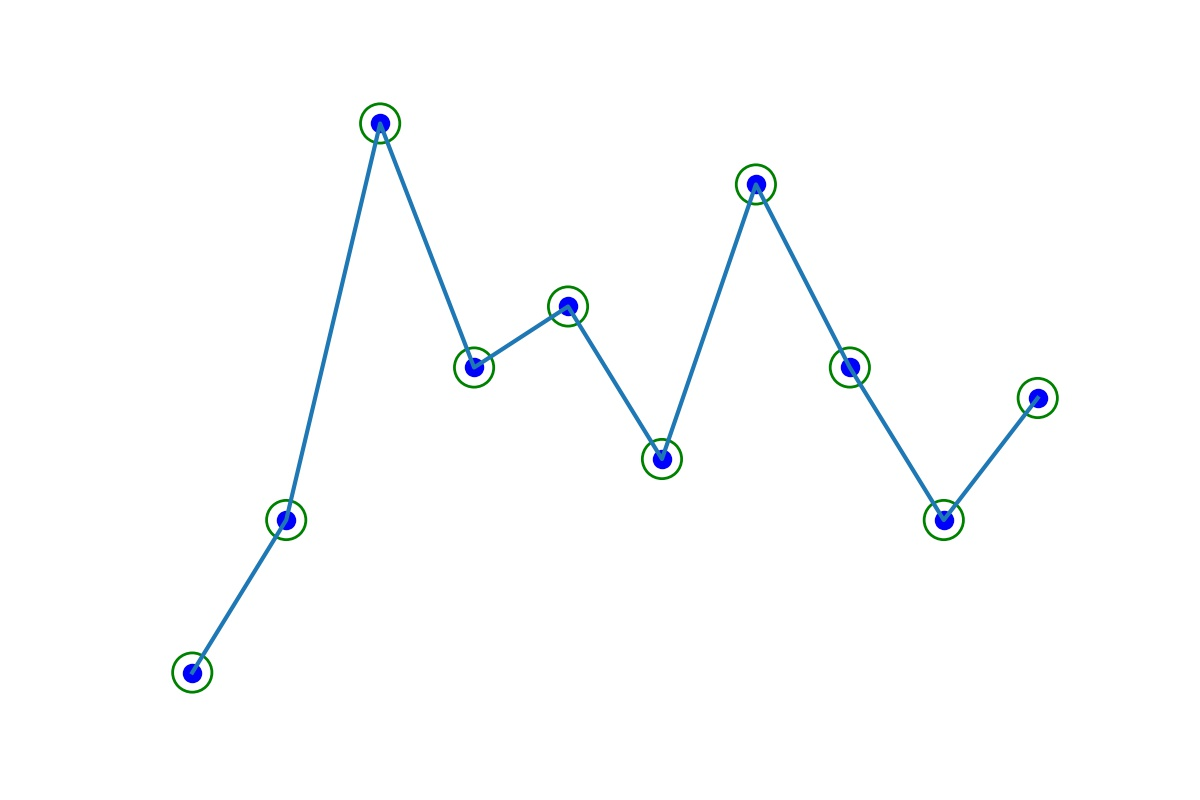
\includegraphics[width=2in]{original.jpg}
        \label{fig:original}
    }
    \subfigure[PPA Result]{
        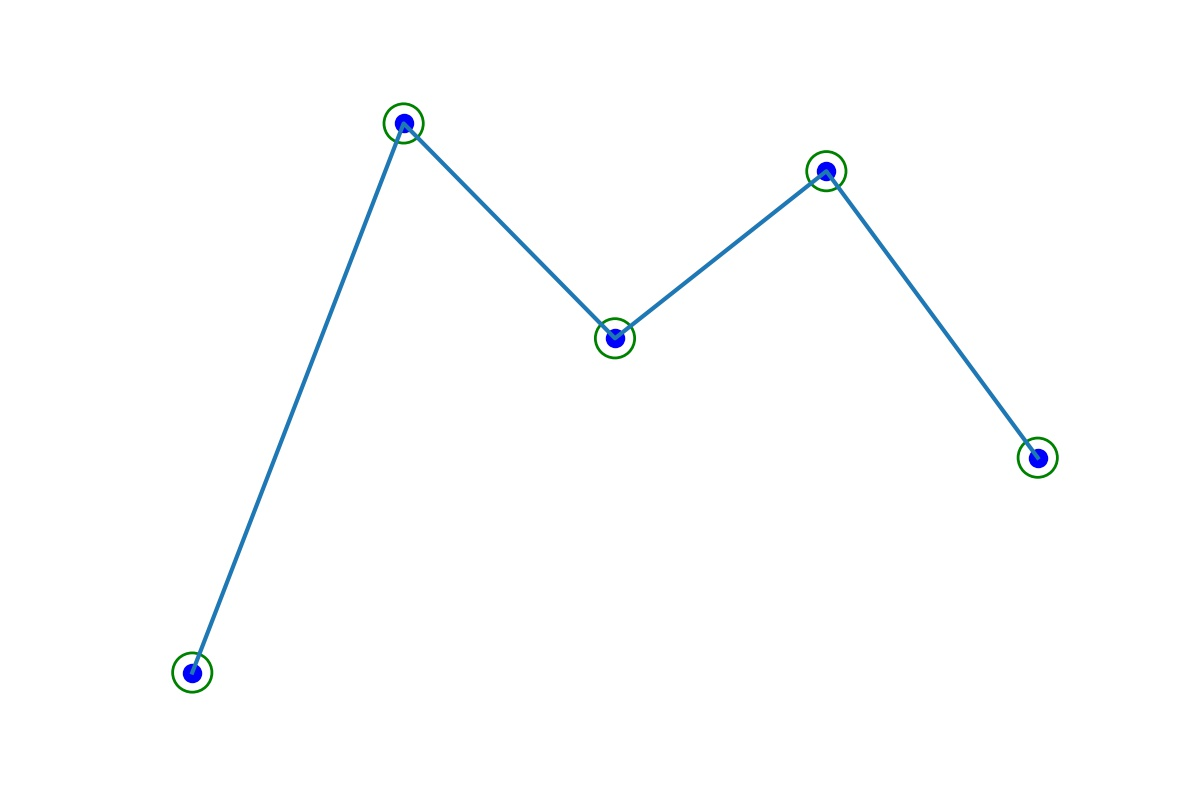
\includegraphics[width=2in]{ppa.jpg}
        \label{fig:ppa}
    }
    \subfigure[PIP Result]{
        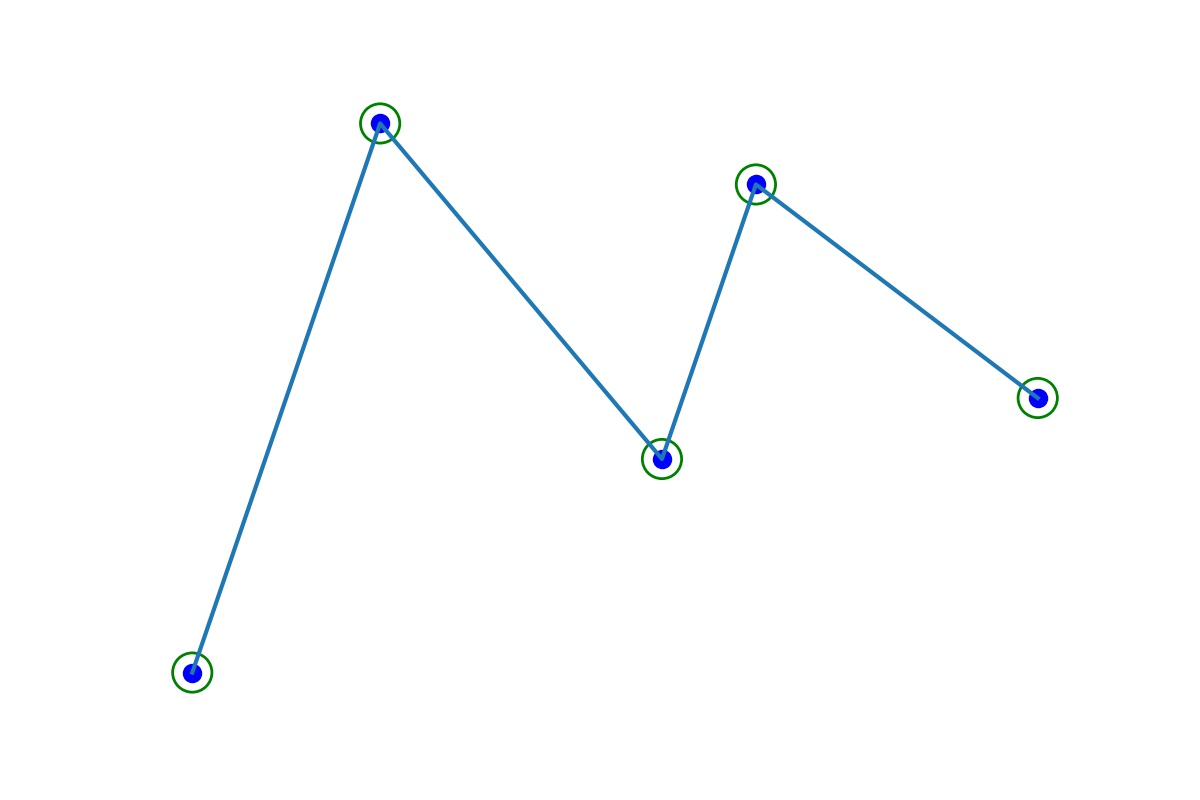
\includegraphics[width=2in]{pip.jpg}
        \label{fig:pip}
    }
    \caption{Compression Results}
\end{figure} 
 
\subsection{Path signature}
Path signature is the core part in rough path theory, it was first studied by \cite{chen1958integration}. As a novel vector representation for sequential data, it has already be used in fields such as financial data analysis \cite{gyurko2013extracting}, handwritten text recognition \cite{xie2016fully}, human action recognition \cite{yang2017developing}, etc. The brief introduction could be: given a sequence (continuous or discrete) $P = (P_1, P_2, \cdots, P_T) \in \mathbb{R}^{T \times D}$, where T is number of points in the sequence, D is the dimension of each data point, let $P_t^i$ denotes the i-th attribute of point $P_t$ $(1\le t\le T, 1 \le i \le D)$, the whole sequence can be represented by n-fold iterated integral over the sequence (n could be infinite). The simplest case is that when $D = 1$, the 1-fold representation of P is a real value defined as:
\begin{equation}
    S(P)_{1,T}^1 = \int_{1 < t \le T}dP_t^1 = P_T^1 - P_1^1
\end{equation}
Similarly, the 2-fold representation is also a real value:
\begin{equation}
    S(P)_{1,T}^{11} = \int_{1 < t \le T} S(P)_{1,T}^1dP_t^1 = \frac{1}{2} (P_T^1 - P_1^1)^2
\end{equation}
The k-fold representation is: 
\begin{equation}
    S(P)_{1,T}^{11\cdots 1} = \frac{1}{k!} (P_T^1 - P_1^1)^k
\end{equation}
The final signature representation of sequence P is the vector $(S(P)_{1,T}^1, S(P)_{1,T}^{11}S(P)_{1,T}^{11\cdots 1}) \in \mathbb{R}^k $ , whose dimension k is the number of fold wanted by users.\\
When D = 2, 1‐fold representation has 2 elements defined as follows:
\begin{equation}
    \begin{aligned}
        S(P)_{1,T}^1 = \int_{1 < t \le T}dP_t^1 = P_T^1 - P_1^1 \\
        S(P)_{1,T}^2 = \int_{1 < t \le T}dP_t^1 = P_T^2 - P_1^2
    \end{aligned}
\end{equation}
2-fold representation has $D^2 = 4$ elements:
\begin{equation}
    \begin{aligned}
        S(P)_{1,T}^{11} & = \int_{1 < t \le T} S(P)_{1,T}^1dP_t^1 = \frac{1}{2} (P_T^1 - P_1^1)^2 \\
        S(P)_{1,T}^{22} & = \int_{1 < t \le T} S(P)_{1,T}^1dP_t^1 = \frac{1}{2} (P_T^2 - P_1^2)^2 \\
        S(P)_{1,T}^{12} & = \int_{1 < t_1 \le T}\int_{1 < t_2 \le T}dP_{t_1}dP_{t_2} \\
        S(P)_{1,T}^{21} & = \int_{1 < t_2 \le T}\int_{1 < t_1 \le T}dP_{t_2}dP_{t_1}
    \end{aligned}
\end{equation}
In general, when D = d, the i-th element of k-fold representation can be seen in eqaution \ref{func:sig1}, where $(n_1,n_2, \cdots, n_k) \in \{1, \cdots, k\}$:
\begin{equation}
    \label{func:sig1}
    S(P)_{1,T}^{n_1,n_2,\cdots, n_k} = \int_{1 < t_k \le T} \cdots \int_{1 < t_3 \le t_4} \int_{1 < t_2 \le t_3}dP_{t_1}^{n_1}dP_{t_2}^{n_2} \cdots dP_{t_k}^{n_k}
\end{equation}
The final signature of the whole path P is the collection of all elements in every fold defined as follows:
\begin{equation}
    \begin{aligned}
        S(P)_{1,T} = (& 1, S(P)_{1,T}^1, \cdots, S(P)_{1,T}^D), \\
        & S(P)_{1,T}^{1,1}, \cdots, S(P)_{1,T}^{2,1}, \cdots, S(P)_{1,T}^{D,1}, \cdots, S(P)_{1,T}^{D,D}, \\
        & S(P)_{1,T}^{1, 1,\cdots, 1}, \cdots, S(P)_{1,T}^{n_1, n_2,\cdots, n_k}, \cdots, S(P)_{1,T}^{D,D,\cdots,D}, \cdots)
    \end{aligned}
\end{equation}
Conventionally, the first term is set to 1. With the increment of fold k, the collection could be infinite. However, in practice, there is no need of using a large k, users can decide the k based the the dimension formula of the final vector: $\omega(D,k) = (D^{k+1} - 1) (D-1)^{-1} $. The truncated elements are regarded as the path signature feature of the original sequence, and then can be used in further analysis.


\subsection{Clustering algorithms}
Clustering is a classical and important task in unsupervised learning. We will use it to find the stcok price moving patterns. Traditional clustering methods can be summarized into following 9 categorizes. Since the main focus of this project is not about clustering algorithms, their technical details are not discussed.
\begin{enumerate}
    \item Partition based: clustering algorithms that assume that the center of data points is the center of the corresponding cluster. Typical algorithms include K-means \cite{macqueen1967some} and K-medoids \cite{park2009simple}.
    \item Hierarchy based: clustering algorithms that generate clusters based on the hierarchical relationship among data points, either in a bottom-up or top-down way. Typical algorithms include BIRCH \cite{zhang1996birch}.
    \item Fuzzy theory based: clustering algorithms that use possibility to represent belonging relationship among objects rather than binary status 0 or 1. One data points could belongs to several clusters at the same time. Typical algorithms include FCM \cite{bezdek1984fcm}, FCS \cite{dave1992adaptive}.
    \item Distribution based: clustering algorithms that assume there were multiple distributions in the original data, and data points sampled from same distribution belong to a same cluster. Typical algorithms include GMM \cite{rasmussen1999infinite}.
    \item Density based: clustering algorithms that assume data points in high density region belong to the same cluster. Typical algorithms include DBSCAN \cite{ester1996density} and Mean-shift \cite{comaniciu2002mean}.
    \item Graph theory based: clustering algorithms that regard data points as nodes and their relationship as edges in a graph. Typical algorithms include CLICK \cite{sharan2000click}.
    \item Grid based: clustering algorithms that transform original data space into a grid structure with fixed size. Typical algorithms include STING \cite{wang1997sting}.
    \item Fractal theory based: clustering algorithms that attempt to divide data points into multiple groups that share some common characters with the original data. Typical algorithms include FC \cite{barbara2000using}.
    \item Model based: clustering algorithms that pre-define a model for each cluster and mathcing data points best fitting for that model. Typical algorithms include COBWEB ]\cite{fisher1987knowledge} and SOM \cite{kohonen1990self}.
\end{enumerate}

Most previous works try to improve the quality of extracted patterns by improving the performance of clustering algorithms. However, we doubt that with a proper data representation method, a simple clustering algorithm can generate acceptable results. Therefore, in this project, we seek to improve the quality of extracted patterns by finding a better representation method of stock price records.